
\chapter{测试}
\label{sec:app1}
\section{公式测试}
\begin{equation}
x_1+x_2=0
 \label{eq:appeq}
\end{equation}

\begin{equation}
    \adddotsbeforeeqnnum%
    \begin{cases}
        \frac{\partial \rho}{\partial t} + \nabla\cdot(\rho\Vector{V}) = 0\\
        \frac{\partial (\rho\Vector{V})}{\partial t} + \nabla\cdot(\rho\Vector{V}\Vector{V}) = \nabla\cdot\Tensor{\sigma}\\
        \frac{\partial (\rho E)}{\partial t} + \nabla\cdot(\rho E\Vector{V}) = \nabla\cdot(k\nabla T) + \nabla\cdot(\Tensor{\sigma}\cdot\Vector{V})
    \end{cases}
    \nonumber
\end{equation}
\begin{equation}
    \adddotsbeforeeqnnum%
    \frac{\partial }{\partial t}\int\limits_{\Omega} u \, \mathrm{d}\Omega + \int\limits_{S} \unitVector{n}\cdot(u\Vector{V}) \, \mathrm{d}S = \dot{\phi}
    \nonumber
\end{equation}
\[
    \begin{split}
        \mathcal{L} \{f\}(s) &= \int _{0^{-}}^{\infty} f(t) e^{-st} \, \mathrm{d}t, \ 
        \mathscr{L} \{f\}(s) = \int _{0^{-}}^{\infty} f(t) e^{-st} \, \mathrm{d}t\\
        \mathcal{F} {\bigl (} f(x+x_{0}) {\bigr )} &= \mathcal{F} {\bigl (} f(x) {\bigr )} e^{2\pi i\xi x_{0}}, \ 
        \mathscr{F} {\bigl (} f(x+x_{0}) {\bigr )} = \mathscr{F} {\bigl (} f(x) {\bigr )} e^{2\pi i\xi x_{0}}
    \end{split}
\]

mathtext: $A,F,L,2,3,5,\sigma$, mathnormal: $A,F,L,2,3,5,\sigma$, mathrm: $\mathrm{A,F,L,2,3,5,\sigma}$.

mathbf: $\mathbf{A,F,L,2,3,5,\sigma}$, mathit: $\mathit{A,F,L,2,3,5,\sigma}$, mathsf: $\mathsf{A,F,L,2,3,5,\sigma}$.

mathtt: $\mathtt{A,F,L,2,3,5,\sigma}$, mathfrak: $\mathfrak{A,F,L,2,3,5,\sigma}$, mathbb: $\mathbb{A,F,L,2,3,5,\sigma}$.

mathcal: $\mathcal{A,F,L,2,3,5,\sigma}$, mathscr: $\mathscr{A,F,L,2,3,5,\sigma}$, boldsymbol: $\boldsymbol{A,F,L,2,3,5,\sigma}$.

vector: $\Vector{\sigma, T, a, F, n}$, unitvector: $\unitVector{\sigma, T, a, F, n}$

matrix: $\Matrix{\sigma, T, a, F, n}$, unitmatrix: $\unitMatrix{\sigma, T, a, F, n}$

tensor: $\Tensor{\sigma, T, a, F, n}$, unittensor: $\unitTensor{\sigma, T, a, F, n}$ 

引用一下附录\ref{sec:app1}里的公式\ref{eq:appeq}式

\section{测试生僻字}

霜蟾盥薇曜灵霜颸妙鬘虚霩淩澌菀枯菡萏泬寥窅冥毰毸濩落霅霅便嬛岧峣瀺灂姽婳愔嫕飒纚棽俪緸冤莩甲摛藻卮言倥侗椒觞期颐夜阑彬蔚倥偬澄廓簪缨陟遐迤逦缥缃鹣鲽憯懔闺闼璀错媕婀噌吰澒洞阛闠覼缕玓瓑逡巡諓諓琭琭瀌瀌踽踽叆叇氤氲瓠犀流眄蹀躞赟嬛茕頔璎珞螓首蘅皋惏悷缱绻昶皴皱颟顸愀然菡萏卑陬纯懿犇麤掱暒 墌墍墎墏墐墒墒墓墔墕墖墘墖墚墛坠墝增墠墡墢墣墤墥墦墧墨墩墪樽墬墭堕墯墰墱墲坟墴墵垯墷墸墹墺墙墼墽垦墿壀壁壂壃壄壅壆坛壈壉壊垱壌壍埙壏壐壑壒压壔壕壖壗垒圹垆壛壜壝垄壠壡坜壣壤壥壦壧壨坝塆圭嫶嫷嫸嫹嫺娴嫼嫽嫾婳妫嬁嬂嬃嬄嬅嬆嬇娆嬉嬊娇嬍嬎嬏嬐嬑嬒嬓嬔嬕嬖嬗嬘嫱嬚嬛嬜嬞嬟嬠嫒嬢嬣嬥嬦嬧嬨嬩嫔嬫嬬奶嬬嬮嬯婴嬱嬲嬳嬴嬵嬶嬷婶嬹嬺嬻嬼嬽嬾嬿孀孁孂娘孄孅孆孇孆孈孉孊娈孋孊孍孎孏嫫婿媚嵭嵮嵯嵰嵱嵲嵳嵴嵵嵶嵷嵸嵹嵺嵻嵼嵽嵾嵿嶀嵝嶂嶃崭嶅嶆岖嶈嶉嶊嶋嶌嶍嶎嶏嶐嶑嶒嶓嵚嶕嶖嶘嶙嶚嶛嶜嶝嶞嶟峤嶡峣嶣嶤嶥嶦峄峃嶩嶪嶫嶬嶭崄嶯嶰嶱嶲嶳岙嶵嶶嶷嵘嶹岭嶻屿岳帋巀巁巂巃巄巅巆巇巈巉巊岿巌巍巎巏巐巑峦巓巅巕岩巗巘巙巚帠帡帢帣帤帨帩帪帬帯帰帱帲帴帵帷帹帺帻帼帽帾帿幁幂帏幄幅幆幇幈幉幊幋幌幍幎幏幐幑幒幓幖幙幚幛幜幝幞帜幠幡幢幤幥幦幧幨幩幪幭幮幯幰幱庍庎庑庖庘庛庝庠庡庢庣庤庥庨庩庪庬庮庯庰庱庲庳庴庵庹庺庻庼庽庿廀厕廃厩廅廆廇廋廌廍庼廏廐廑廒廔廕廖廗廘廙廛廜廞庑廤廥廦廧廨廭廮廯廰痈廲廵廸廹廻廼廽廿弁弅弆弇弉弖弙弚弜弝弞弡弢弣弤弨弩弪弫弬弭弮弰弲弪弴弶弸弻弼弽弿彖彗彘彚彛彜彝彞彟彴彵彶彷彸役彺彻彽彾佛徂徃徆徇徉后徍徎徏径徒従徔徕徖徙徚徛徜徝从徟徕御徢徣徤徥徦徧徨复循徫旁徭微徯徰徱徲徳徴徵徶德徸彻徺忁忂惔愔忇忈忉忔忕忖忚忛応忝忞忟忪挣挦挧挨挩挪挫挬挭挮挰掇授掉掊掋掍掎掐掑排掓掔掕挜掚挂掜掝掞掟掠采探掣掤掦措掫掬掭掮掯掰掱掲掳掴掵掶掸掹掺掻掼掽掾掿拣揁揂揃揅揄揆揇揈揉揊揋揌揍揎揑揓揔揕揖揗揘揙揤揥揦揧揨揫捂揰揱揲揳援揵揶揷揸揻揼揾揿搀搁搂搃搄搅搇搈搉搊搋搌搎搏搐搑搒摓摔摕摖摗摙摚摛掼摝摞摠摡斫斩斮斱斲斳斴斵斶斸旪旫旮旯晒晓晔晕晖晗晘晙晛晜晞晟晠晡晰晣晤晥晦晧晪晫晬晭晰晱晲晳晴晵晷晸晹晻晼晽晾晿暀暁暂暃暄暅暆暇晕晖暊暋暌暍暎暏暐暑暒暓暔暕暖暗旸暙暚暛暜暝暞暟暠暡暣暤暥暦暧暨暩暪暬暭暮暯暰昵暲暳暴暵

\section{图表测试}
\begin{equation}
x_1+x_2=1
 \label{eq:appeq2}
\end{equation}
\subsection{图测试}
\begin{figure}[!htbp]
    \centering
    \begin{subfigure}[b]{0.35\textwidth}
      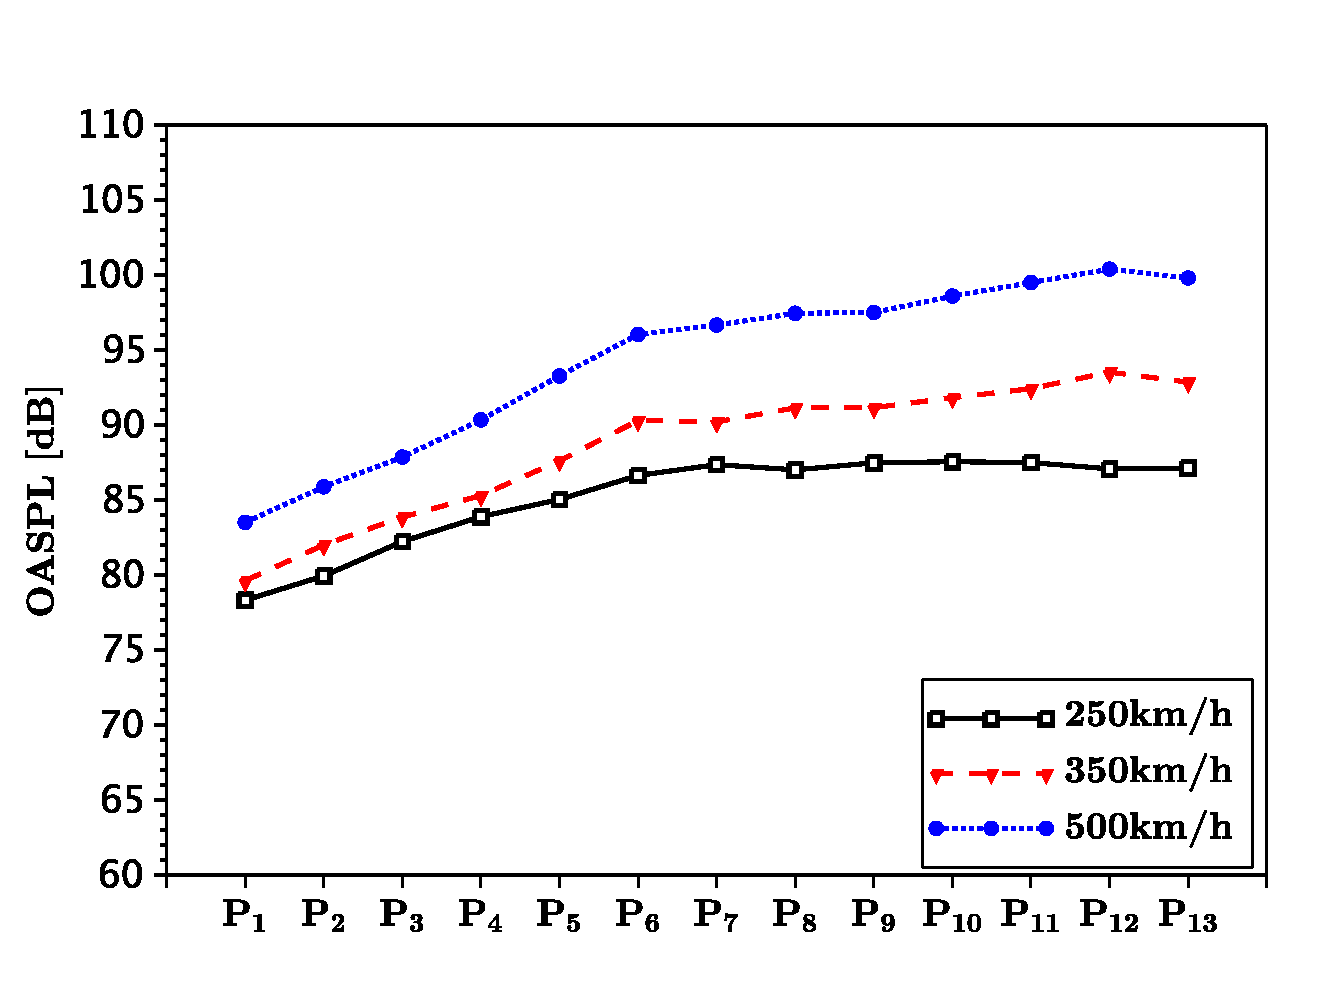
\includegraphics[width=\textwidth]{oaspl_a}
      \caption{}
      \label{fig:oaspl_a}
    \end{subfigure}%
    ~% add desired spacing
    \begin{subfigure}[b]{0.35\textwidth}
      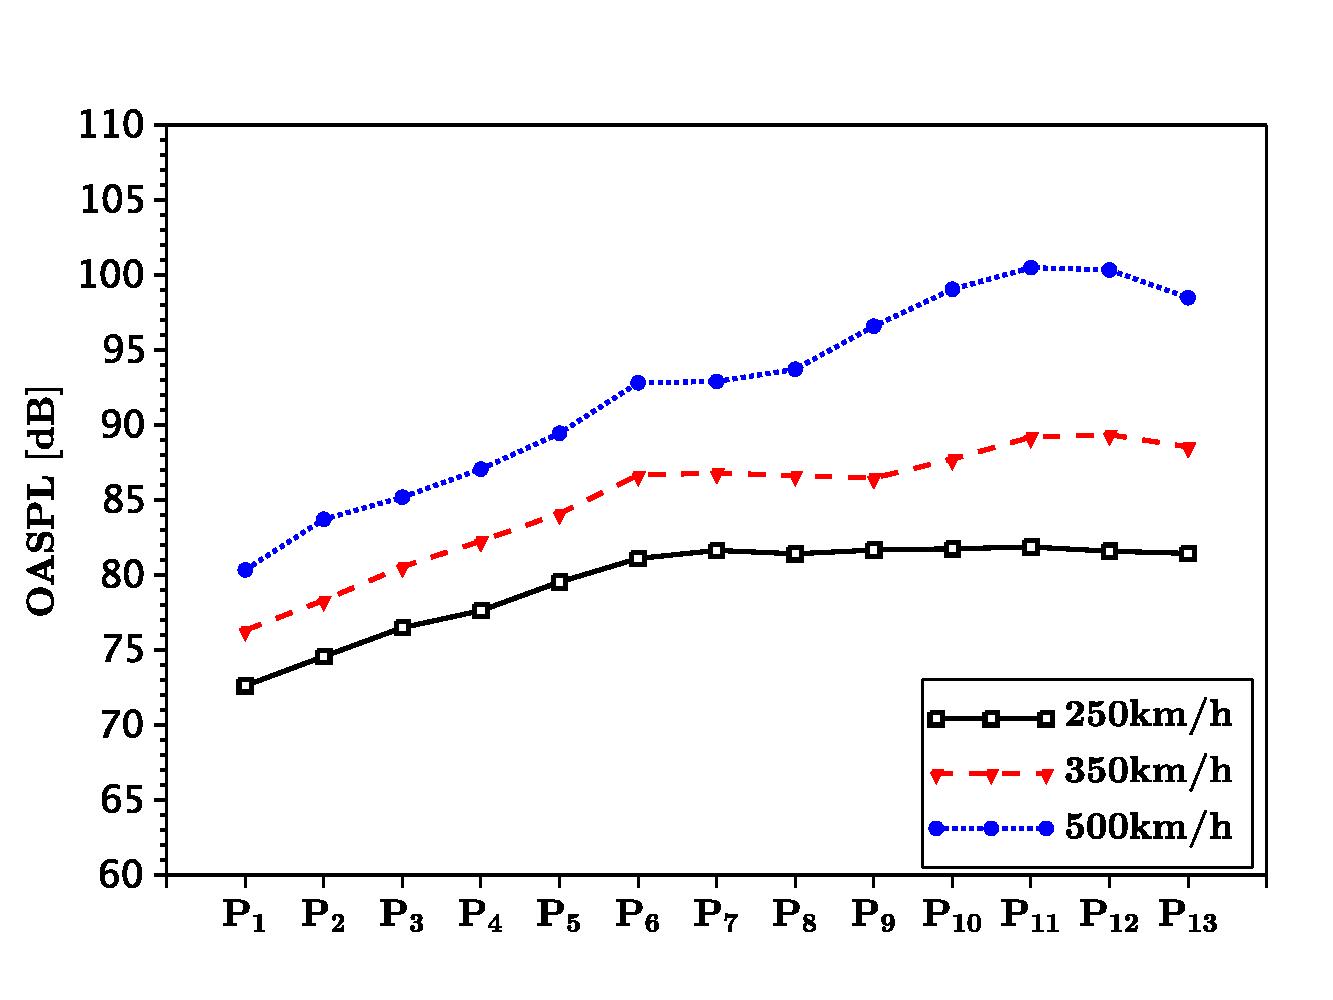
\includegraphics[width=\textwidth]{oaspl_b}
      \caption{}
      \label{fig:oaspl_b}
    \end{subfigure}
    \\% line break
    \begin{subfigure}[b]{0.35\textwidth}
      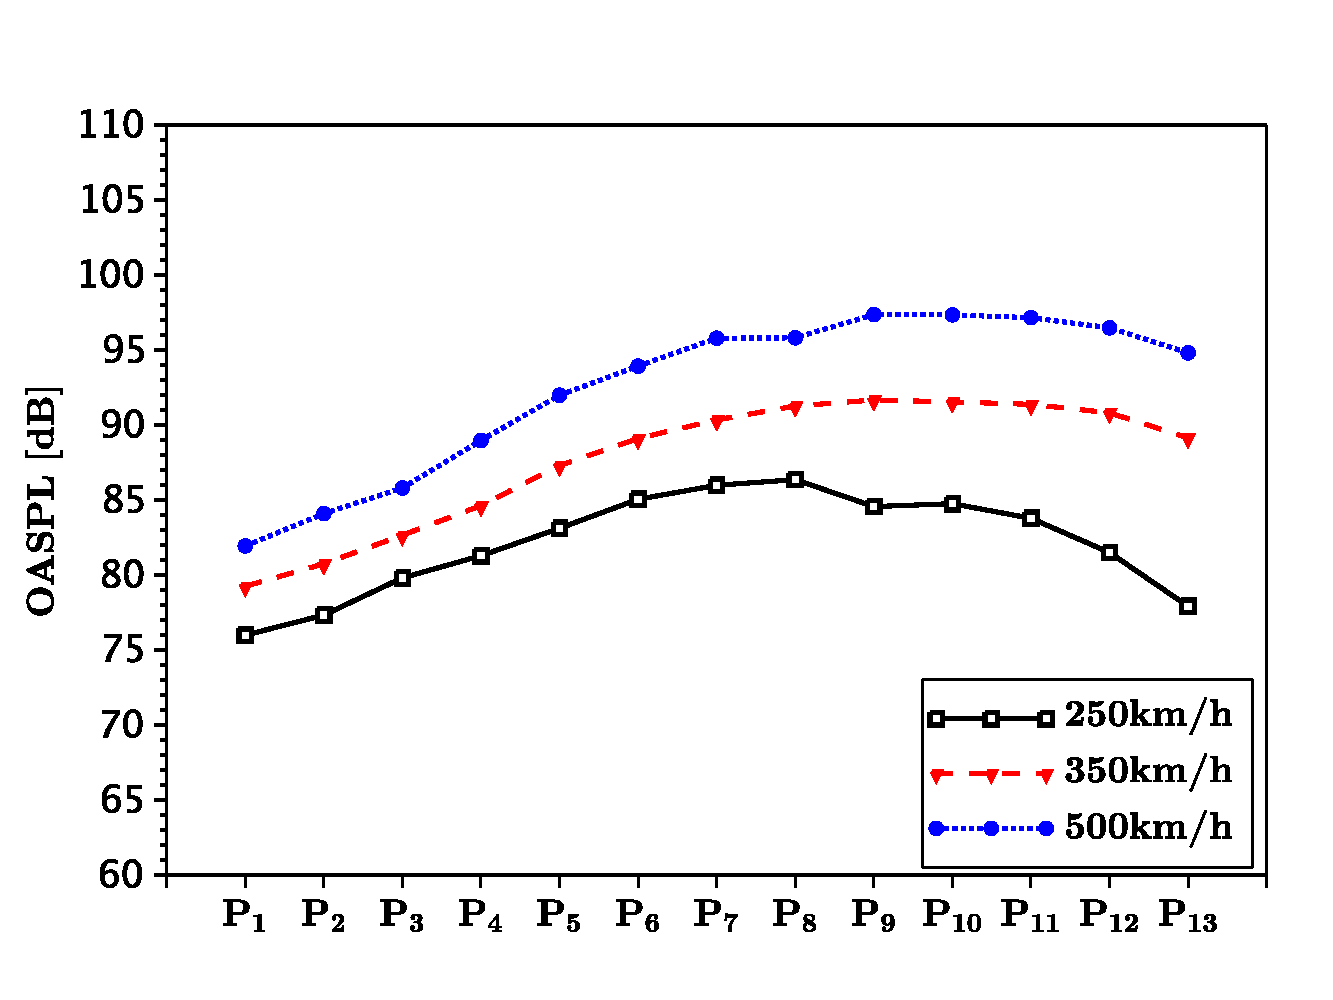
\includegraphics[width=\textwidth]{oaspl_c}
      \caption{}
      \label{fig:oaspl_c}
    \end{subfigure}%
    ~% add desired spacing
    \begin{subfigure}[b]{0.35\textwidth}
      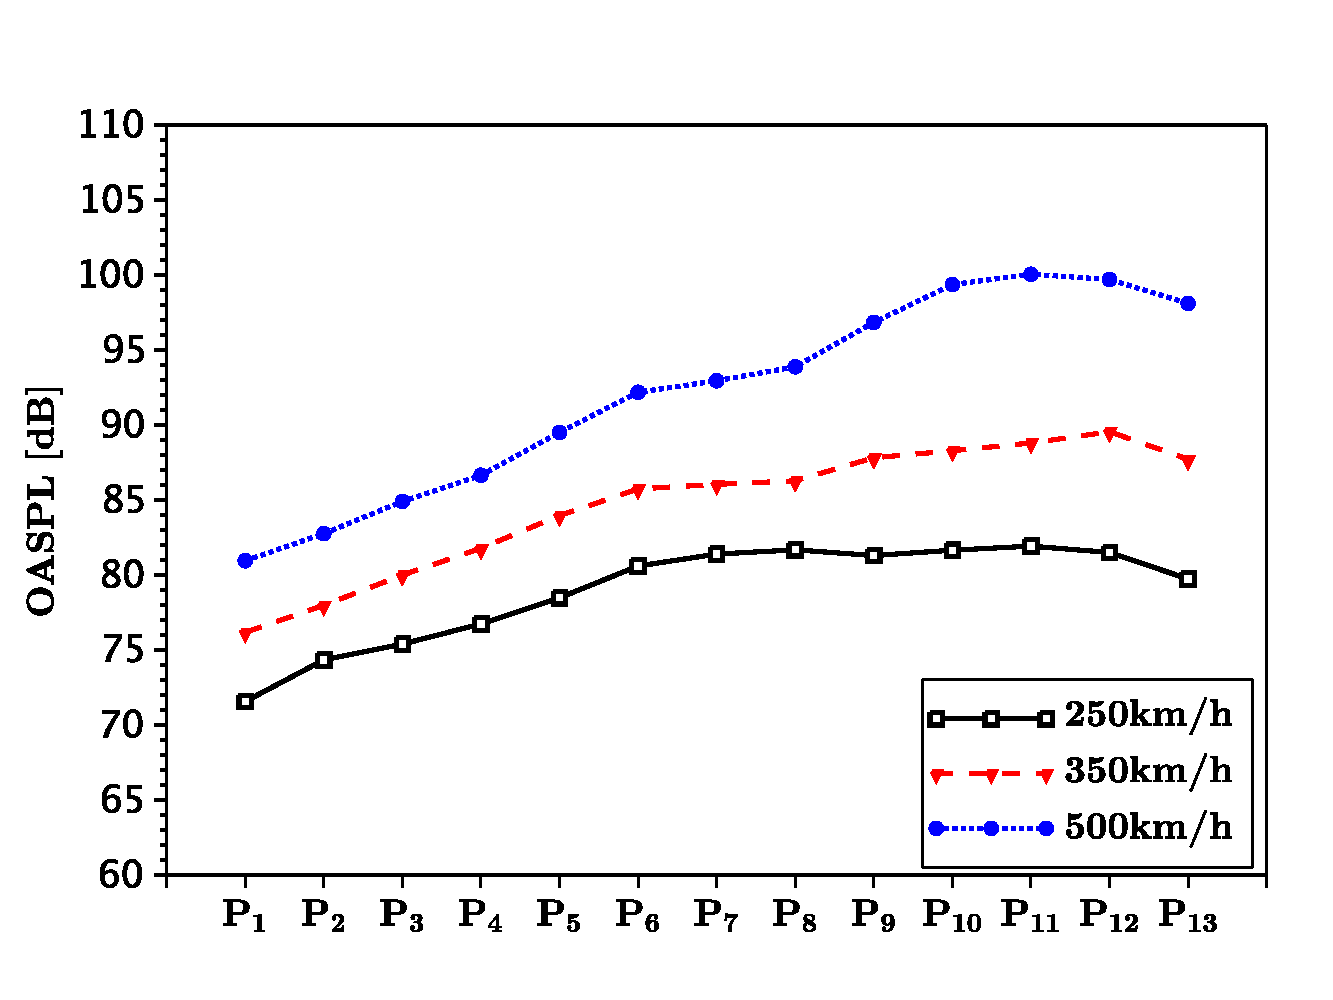
\includegraphics[width=\textwidth]{oaspl_d}
      \caption{}
      \label{fig:oaspl_d}
    \end{subfigure}
    \caption{多子图测试}%{\quad A test for multi-subfig}
    \label{fig:oaspla}
\end{figure}

这里见\ref{fig:caspla}.

\subsection{表测试}

请见\ref{tab:sampleA}。
\begin{table}[!htbp]
    \caption{这是一个样表}%{\quad This is a sample table}
    \label{tab:sampleA}
    \centering
    \footnotesize% fontsize
    \setlength{\tabcolsep}{4pt}% column separation
    \renewcommand{\arraystretch}{1.2}%row space 
    \begin{tabular}{lcccccccc}
        \hline
        行号 & \multicolumn{8}{c}{跨多列的标题}\\
        %\cline{2-9}% partial hline from column i to column j
        \hline
        Row 1 & $1$ & $2$ & $3$ & $4$ & $5$ & $6$ & $7$ & $8$\\
        Row 2 & $1$ & $2$ & $3$ & $4$ & $5$ & $6$ & $7$ & $8$\\
        Row 3 & $1$ & $2$ & $3$ & $4$ & $5$ & $6$ & $7$ & $8$\\
        Row 4 & $1$ & $2$ & $3$ & $4$ & $5$ & $6$ & $7$ & $8$\\
        \hline
    \end{tabular}
\end{table}

\chapter{凑数用的}

\section{测试二}